\documentclass[12pt,a4paper]{article}
\usepackage{amsmath}
\usepackage{graphicx}
\usepackage{hyperref}
\usepackage{float}
\usepackage{enumerate}
\usepackage{amssymb}

\title{COL 774: Assignment 2 Report}
\author{Parth Thakur, 2021CS50615}
\date{Wednesday Oct 4, 2023}

\begin{document}
\maketitle

\section{Text Classification}
\subsection{Naïve Bayes Multiclass Classification}
\subsubsection{Accuracy Report}
\begin{itemize}
    \item Training: 80.23 percent  
    \item Validation: 69.96 percent
\end{itemize}


\subsubsection{Word Cloud Construction}
\begin{figure}[H]
\centering
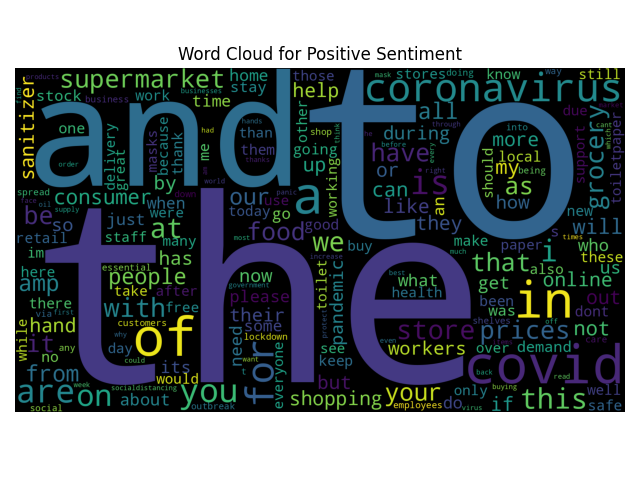
\includegraphics[width=0.8\textwidth]{Assignment 2/q1/wordcloud_Positive.png}
\end{figure}

\begin{figure}[H]
\centering
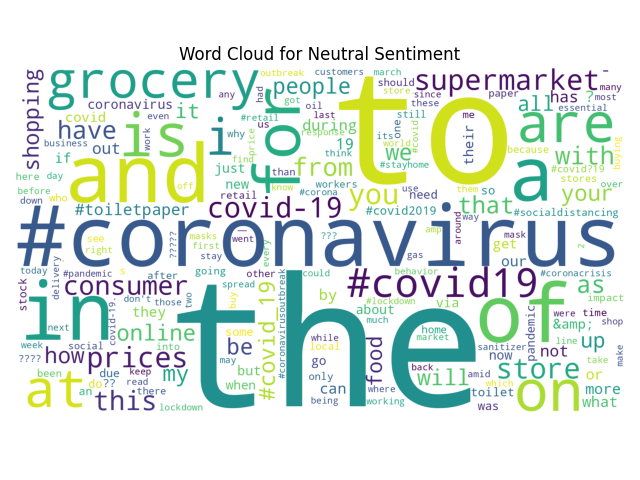
\includegraphics[width=0.8\textwidth]{Assignment 2/q1/wordcloud_Neutral.png}
\end{figure}

\begin{figure}[H]
\centering
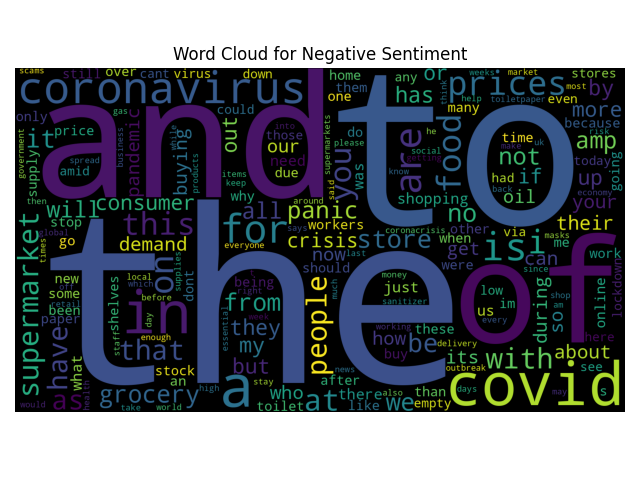
\includegraphics[width=0.8\textwidth]{Assignment 2/q1/wordcloud_Negative.png}
\end{figure}


\subsection{Random and Positive Baseline Accuracy}
\begin{itemize}
    \item Random:
    \begin{itemize}
        \item Training: 33.32 percent
        \item Validation: 32.82 percent
    \end{itemize}

    \item Positive:
    \begin{itemize}
        \item Training: 43.84 percent
        \item Validation: 43.85 percent
    \end{itemize}
\end{itemize}

Comparing to the Naive Bayes Classifier I have created, as expected, it performs better than both Random and Positive Prediction.

\begin{table}[h]
    \centering
    \begin{tabular}{|l|c|c|}
    \hline
    \textbf{Method} & \textbf{Training Accuracy} & \textbf{Validation Accuracy} \\
    \hline
    Random & 33.32\% & 32.82\% \\
    \hline
    Positive & 43.84\% & 43.85\% \\
    \hline
    Naïve Bayes (Accuracy Report) & 80.23\% & 69.96\% \\
    \hline
    \end{tabular}
    \caption{Comparison of different methods for text classification.}
    \label{tab:comparison}
\end{table}


\subsection{Confusion Matrix}

\subsubsection{Naive Bayes}

\textbf{Training Set}
\begin{center}
\begin{tabular}{|c|c|c|c|}
\hline
 & Positive & Negative & Neutral \\
\hline
Positive & 14770 & 1565 & 267 \\
\hline
Negative & 1699 & 12252 & 215 \\
\hline
Neutral & 2238 & 1500 & 3358 \\
\hline
\end{tabular}
\end{center}

\textbf{Validation Set}
\begin{center}
\begin{tabular}{|c|c|c|c|}
\hline
 & Positive & Negative & Neutral \\
\hline
Positive & 1196 & 226 & 22 \\
\hline
Negative & 254 & 952 & 26 \\
\hline
Neutral & 290 & 171 & 156 \\
\hline
\end{tabular}
\end{center}

\subsubsection{Random}

\textbf{Training Set}
\begin{center}
\begin{tabular}{|c|c|c|c|}
\hline
 & Positive & Negative & Neutral \\
\hline
Positive & 5575 & 5528 & 5499 \\
\hline
Negative & 4834 & 4689 & 4643 \\
\hline
Neutral & 2407 & 2337 & 2352 \\
\hline
\end{tabular}
\end{center}

\textbf{Validation Set}
\begin{center}
\begin{tabular}{|c|c|c|c|}
\hline
 & Positive & Negative & Neutral \\
\hline
Positive & 465 & 505 & 474 \\
\hline
Negative & 401 & 427 & 404 \\
\hline
Neutral & 205 & 223 & 189 \\
\hline
\end{tabular}
\end{center}

\subsubsection{Positive}

\textbf{Training Set}
\begin{center}
\begin{tabular}{|c|c|c|c|}
\hline
 & Positive & Negative & Neutral \\
\hline
Positive & 16602 & 0 & 0 \\
\hline
Negative & 14166 & 0 & 0 \\
\hline
Neutral & 7096 & 0 & 0 \\
\hline
\end{tabular}
\end{center}

\textbf{Validation Set}
\begin{center}
\begin{tabular}{|c|c|c|c|}
\hline
 & Positive & Negative & Neutral \\
\hline
Positive & 1444 & 0 & 0 \\
\hline
Negative & 1232 & 0 & 0 \\
\hline
Neutral & 617 & 0 & 0 \\
\hline
\end{tabular}
\end{center}



\begin{enumerate}
	\item Naive Bayes:

\begin{itemize}
		\item Training Set: The category with the highest value on the diagonal is Positive with 14770 correct predictions.
		\item Validation Set: The category with the highest value on the diagonal is Positive with 1196 correct predictions.
\end{itemize}

	\item Random:

\begin{itemize}
		\item Training Set: The category with the highest value on the diagonal is Positive with 5575 correct predictions.
		\item Validation Set: The category with the highest value on the diagonal is Positive with 465 correct predictions.
\end{itemize}

	\item Positive:

\begin{itemize}
		\item Training Set: The category with the highest value on the diagonal is Positive with 16602 correct predictions.
		\item Validation Set: The category with the highest value on the diagonal is Positive with 1444 correct predictions.
\end{itemize}

\end{enumerate}
The highest value on the diagonal entry indicates that this category was the most accurately predicted among the three. For all three methods (Naive Bayes, Random, and Positive), the "Positive" category has the highest number of correctly predicted instances. This means that the model is best at correctly identifying positive samples.




\subsection{Stopword Removal and Stemming}
\subsubsection{Data Transformation}
Stop Word removal is performed using the set of English stop words in the nltk corpus. Stemming is done using PorterStemmer from nltk.stem.

\subsubsection{Word Clouds}
\begin{figure}[H]
\centering
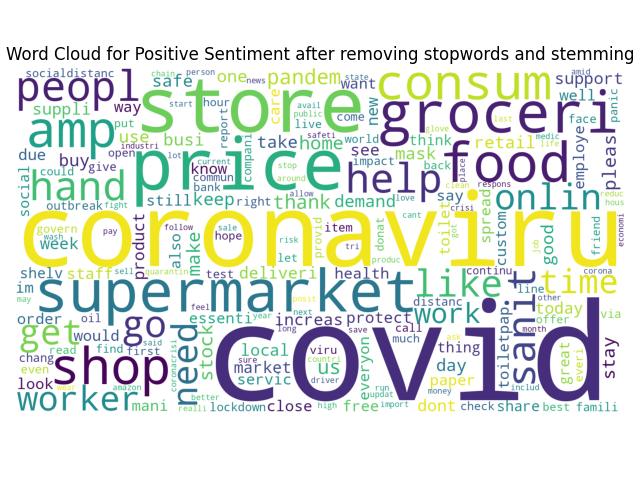
\includegraphics[width=0.8\textwidth]{Assignment 2/q1/wordcloud_Positive_stemming_and_removeStopwords.png}
\end{figure}

\begin{figure}[H]
\centering
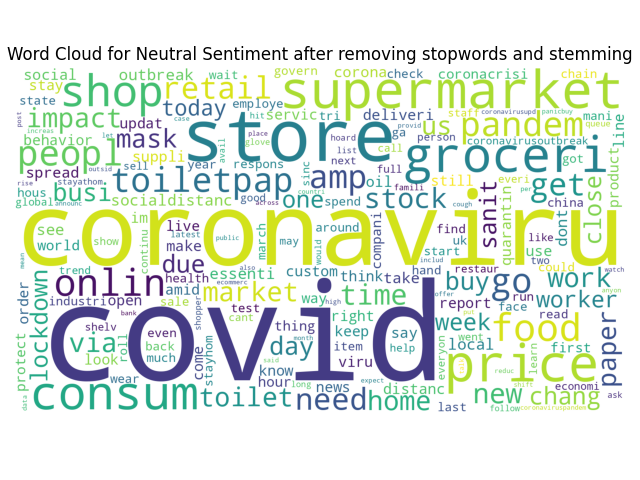
\includegraphics[width=0.8\textwidth]{Assignment 2/q1/wordcloud_Neutral_stemming_and_removeStopwords.png}
\end{figure}

\begin{figure}[H]
\centering
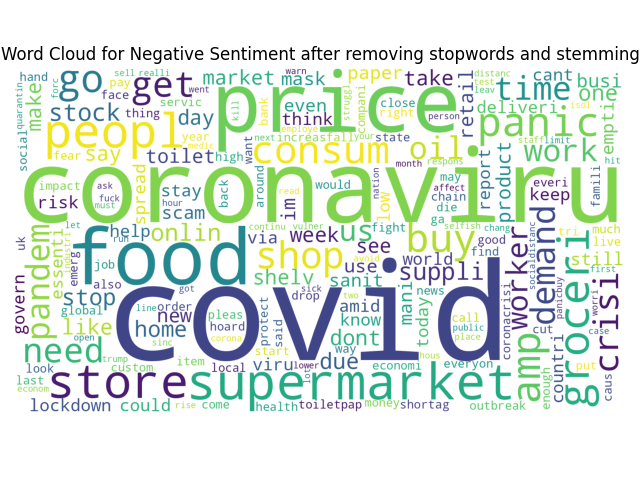
\includegraphics[width=0.8\textwidth]{Assignment 2/q1/wordcloud_Negative_stemming_and_removeStopwords.png}
\end{figure}

\subsubsection{Model Accuracy}
\begin{itemize}
    \item Training: 73.46 percent
    \item Validation: 22.98 percent
\end{itemize}

\subsubsection{Observations}
% Write your answer for part 1(d)iv here.

\subsection{Feature Engineering}
% Write your answers for part 1(e) here.

\subsection{Domain Adaptation}
% Write your answers for part 1(f) here.

\section{Image Classification}
\subsection{Binary Classification}
\subsubsection{Using CVXOPT}
% Write your answers for part 2(a) here.

\subsubsection{Using scikit-learn SVM function}
% Write your answers for part 2(b) here.

\subsection{Multi-Class Image Classification}
\subsubsection{One-vs-One Multi-Class SVM}
% Write your answer for part 2(a)i here.

\subsubsection{Using scikit-learn SVM function}
% Write your answers for part 2(b) here.

\subsubsection{Confusion Matrix and Observations}
% Write your answers for part 2(c) here.

\subsubsection{Validation and Cross-Validation}
% Write your answers for part 2(d) here.

\section*{Conclusions}
% Summarize your findings and observations here.

\end{document}
